\section{The Background Channels}\label{sec:bkg}
We define background as anything that is not of interest and that mimics the signals of new physics considered. 
As will be further explained in  later sections, we will explicitly demand a 3-lepton final-state in all collisions 
considered in the analysis. This will remove a lot of background, but not all. Due to the imperfect nature of the 
reconstruction of events, a demand for 3-lepton final-state will not be without errors. This leaves room for more 
variation in the background than one might expect. In this section I will cover the channels\footnote{By channels,
we refer to the physical diversity which could lead to a specific final-state. Often this refers to 
the different particles which mediates the process from initial- to final-state.} which will 
be of importance during the analysis. I will also discuss which background channels are the hardest 
to reduce in a potential new physics signal region, also called the irreducible background. These are 
channels that exhibit similar trends/distribution in the features. Note that the sections bellow
are listed by contribution to the 3-lepton final-state data (from most to least).  
\\
The processes I will describe in the section to come, are classified similarly to how they were classified in the original 
\ac{MC} simulated data I was given. For the sake of making several of the figures in the thesis more readable, I decided 
to merge several of the classifications. Diboson(llll), diboson(lll) and diboson(ll) are in later figures, categorized as 
simply diboson. Similarly, the three smallest processes, triboson, W-jets and Higgs, are all merged to the same category, $Others$.
\subsection{Z-jets}
The Z-jets channel is the largest contribution in all the data. The channel consists of all events
resulting in a Z-boson alongside jets. In the cases the Z-boson decays into two leptons, the additional 
jet acts as a fake lepton and the channel classifies as a 3-lepton final state. In figure \ref{fig:z_pjets} 
I have written the Feynman diagram of an example of such a channel. The figure shows a quark-antiquark leading 
to a Z-boson and gluon. The Z boson decays into two leptons (normally 
$e^-e^+$ or $\mu^- \mu^+$) and the gluon hadronises as a jet of hadrons which may obtain a b-hadron leading to a 
fake lepton. 

\subsection{Diboson (lll)}
Dibson channels are defined as channels resulting in two bosons. In the case of (lll), the dibosons
decay into a total of three leptons. In figure \ref{fig:wz} I have drawn the Feynman diagram of an 
example of such a channel. The figure shows a W- and Z-boson production through a quark-antiquark pair.
The W-boson decays into a lepton with missing energy\footnote{Neutrinos very rarely interact
with anything, making them almost impossible to detect. We therefore refer to neutrinos as missing energy.}
and the Z-boson decays into a pair of leptons. 

\subsection{$t\bar{t}$}\label{subsec:ttbar}
The $t\bar{t}$ channel is defined as a proton-proton collision resulting in a top quark-antiquark production 
through the strong interaction. In figure \ref{fig:ttbar} I have drawn a Feynman diagram of an example of such 
a channel. The figure shows gluon-gluon fusion producing a pair of top quarks. The top-antitop pair decay into 
a bottom-quark and a W boson. The channel constitutes a background when both W bosons decay into a charged and a 
neutral lepton and one of the b-quarks leads to a fake lepton.

\subsection{Diboson (llll)}
In the case of diboson (llll), the channel refers to events resulting in two Z-bosons which decay 
into four leptons. In figure \ref{fig:zz} I have drawn a Feynman diagram of an example of 
such a diagram. The figure shows a quark-antiquark pair annihilating into two Z-bosons.
The two Z-bosons decay into two pairs of leptons. This process constitutes a background when one 
of the leptons is not reconstructed in the detector.


\subsection{Top Others}
The top other channel is similar to the $t\bar{t}$ channel, in that it results in top quarks. The main difference between 
the two, is that the top other process does not produce a top quark-antiquark pair through strong interaction of quarks. 
In figure \ref{fig:topOthers} I have drawn an example of a top other process, where a top quark-antiquark pair is produced 
from a bottom quark-antiquark pair collision mediated through a W boson. From this point, the top quark-antiquark pair decays 
to a similar state as described in section \ref{subsec:ttbar}. 

\subsection{Single Top}
The single top channel, similarly to top other and the $t\bar{t}$ channel also produces a top quark, but in the case of single top 
it only produces the one. In figure \ref{fig:topOthers} I have drawn the Feynman diagram of such a channel. The Feynman diagram displays a
top quark produced through the strong interaction of a bottom quark and a gluon. The top quark is produced through the interaction with a W boson 
which decays into a charged-neutral lepton pair and the top quark decays to a W boson and bottom quark. 
\subsection{Diboson (ll)}
The diboson(ll), similarly to diboson(llll) produces two bosons, but instead of ending in a four lepton final state, ends in a two lepton final state.
Figure \ref{fig:ww}, displays the Feynman diagram of a diboson(ll) process where a W-pair is produced through the annihilation of two fermions through 
a charged boson. To produce the two lepton final state, the two bosons must each decay into a charged-neutral lepton pair. 
\subsection{Triboson}
The triboson channel is defined as a proton-proton collision producing three bosons.  In figure \ref{fig:zzz}, I have drawn a Feynman diagram 
displaying an example of a triboson process. The Feynman diagram shows a quark-antiquark pair annihilating to three bosons, two W and one Z. The Z-boson decays 
to a pair of leptons, and the two W bosons each decay into a charged-neutral lepton pair resulting in a 4-lepton final state with missing energy.
\subsection{W-jets}
The W-jets is defined as a proton-proton collision producing a W boson alongside jets. In figure \ref{fig:w_pjets} I have drawn an example 
of a Feynman diagram for a W-jets processes. The Feynman diagram displays a pair of quarks colliding to form a W boson alongside a gluon. The gluon decays 
into a bottom quark-antiquark pair and the W boson decays into a charged-neutral lepton pair. Given that this Feynman diagram only produces the one lepton, it 
relies heavily on poor reconstruction, and is hence quite rare.
\subsection{Higgs}
Finally, we have the Higgs process, which is defined as proton-proton collision producing a Higgs boson. The Higgs boson is relatively heavy (ca. 125Gev), and is therefore
the rarest process in the data set. In figure \ref{fig:h}, I have drawn a Feynman diagram of a collision producing a Higgs boson. The Feynman diagram displays a gluon pair annihilation
through exchanging a virtual top quark, and producing a virtual top quark-antiquark pair. The latter pair, annihilate, producing a Higgs boson, which quickly (due to its mass) into a 
pair of Z bosons. The Z boson pair then further decay into a total of 4 leptons. 

\begin{figure}
    \makebox[\linewidth][c]{%
        \begin{subfigure}{.5\textwidth}
            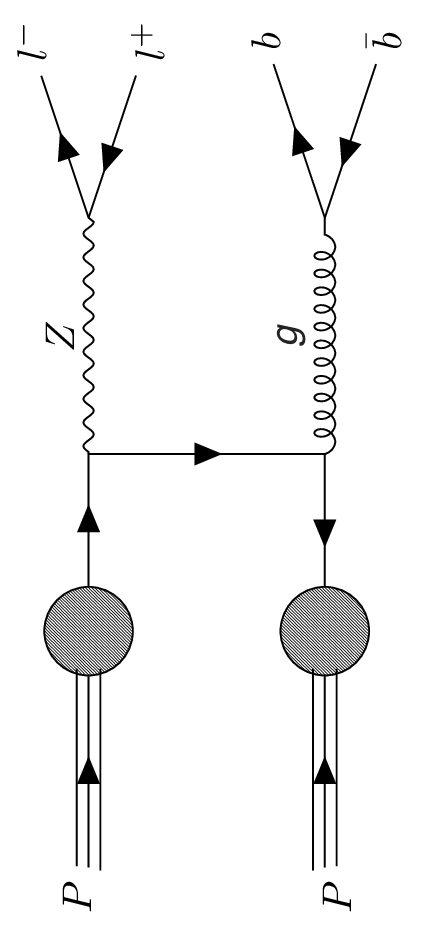
\includegraphics[width=0.45\textwidth, angle = -90]{Figures/FDiagrams/Z_pjets.png}
            \caption{}
            \label{fig:z_pjets}
        \end{subfigure}
        \hspace{1.5cm}
        \begin{subfigure}{.5\textwidth}
            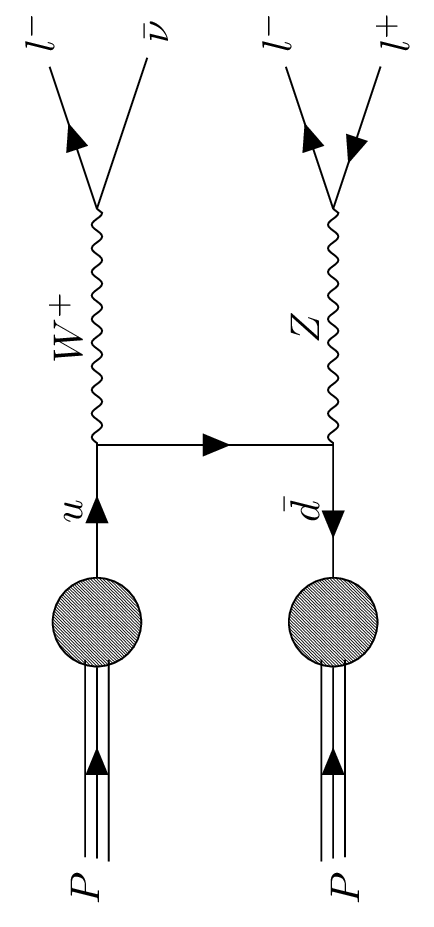
\includegraphics[width=0.45\textwidth, angle = -90]{Figures/FDiagrams/wz.png}
            \caption{}
            \label{fig:wz}
        \end{subfigure}
    }
    \\
    \newline
    \makebox[\linewidth][c]{%
        \begin{subfigure}{.5\textwidth}
            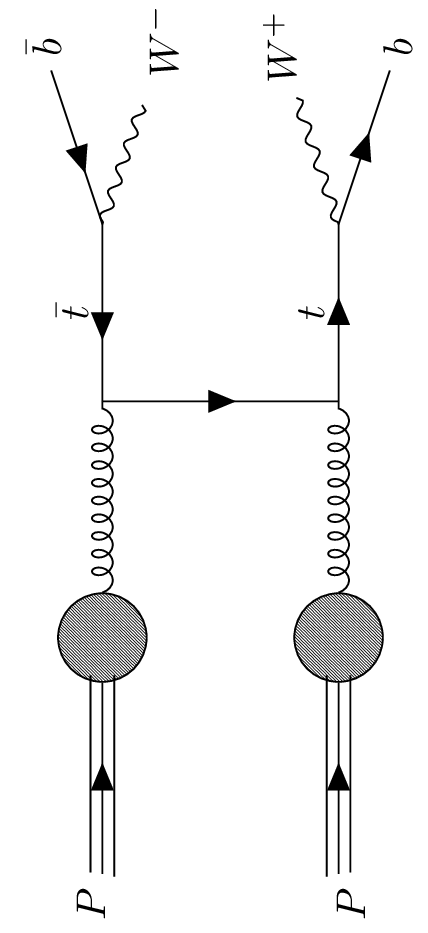
\includegraphics[width=0.45\textwidth, angle = -90]{Figures/FDiagrams/ttbar.png}
            \caption{}
            \label{fig:ttbar}
        \end{subfigure}
        \hspace{1.5cm}
        \begin{subfigure}{.5\textwidth}
            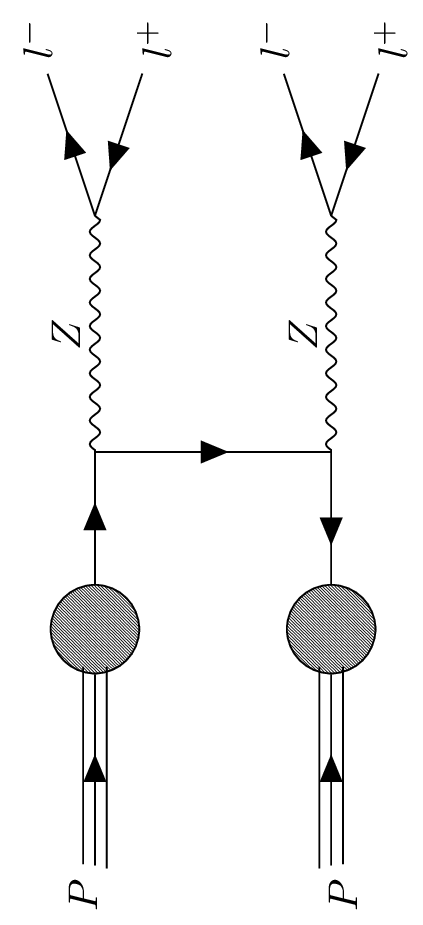
\includegraphics[width=0.45\textwidth, angle = -90]{Figures/FDiagrams/zz.png}
            \caption{}
            \label{fig:zz}
        \end{subfigure}
    }
    \\
    \newline
    \makebox[\linewidth][c]{%
        \begin{subfigure}{.5\textwidth}
            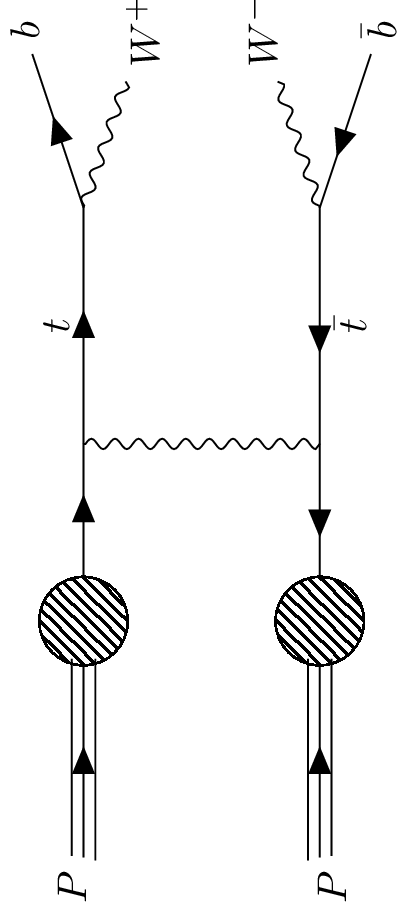
\includegraphics[width=0.5\textwidth, angle = -90]{Figures/FDiagrams/topOther.png}
            \caption{}
            \label{fig:topOthers}
        \end{subfigure}
        \hspace{1.5cm}
        \begin{subfigure}{.5\textwidth}
            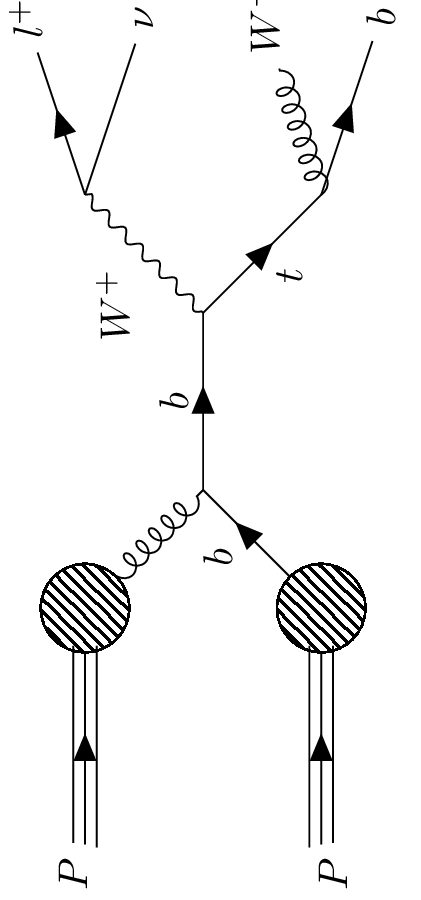
\includegraphics[width=0.45\textwidth, angle = -90]{Figures/FDiagrams/singleTop.png}
            \caption{}
            \label{fig:singleTop}
        \end{subfigure}
    }
    \\
    \newline
    \makebox[\linewidth][c]{%
        \begin{subfigure}{.5\textwidth}
            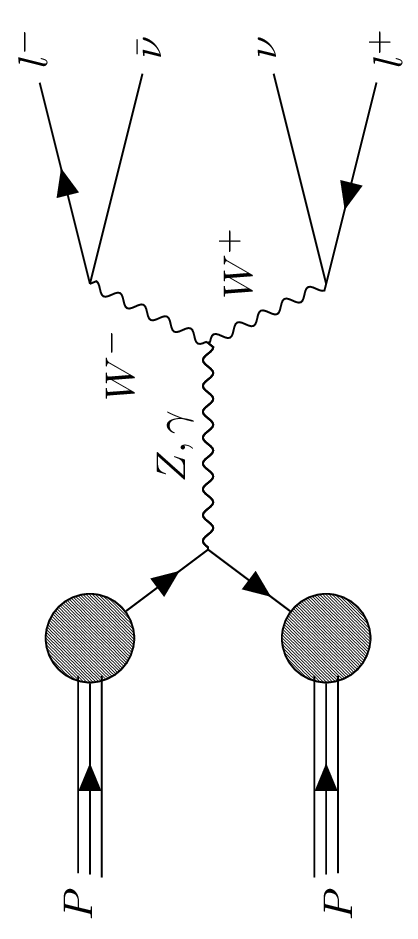
\includegraphics[width=0.45\textwidth, angle = -90]{Figures/FDiagrams/ww.png}
            \caption{}
            \label{fig:ww}
        \end{subfigure}
        \hspace{1.5cm}
        \begin{subfigure}{.5\textwidth}
            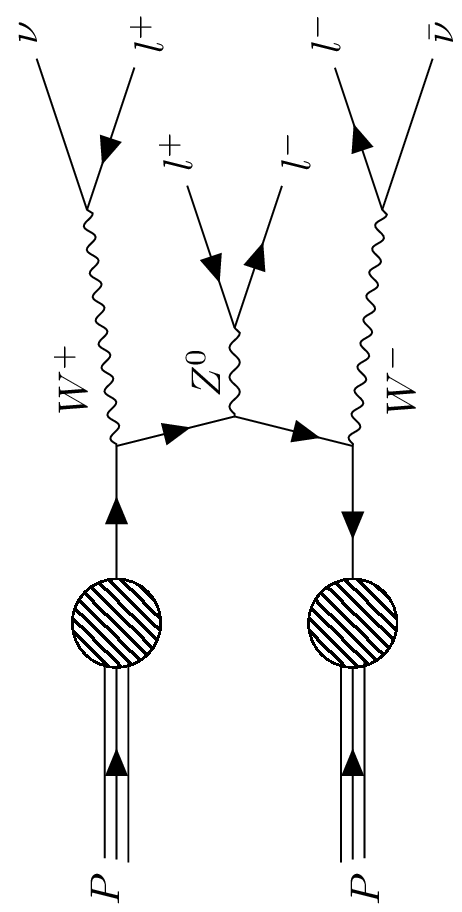
\includegraphics[width=0.46\textwidth, angle = -90]{Figures/FDiagrams/WZW.png}
            \caption{}
            \label{fig:zzz}
        \end{subfigure}
    }
    \\
    \newline
    \makebox[\linewidth][c]{%
        \begin{subfigure}{.5\textwidth}
            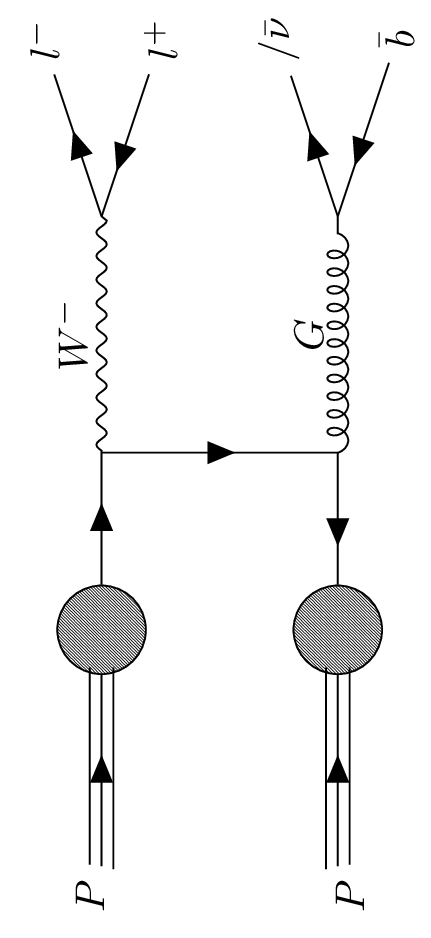
\includegraphics[width=0.45\textwidth, angle = -90]{Figures/FDiagrams/w_pjets.png}
            \caption{}
            \label{fig:w_pjets}
        \end{subfigure}
        \hspace{1.1cm}
        \begin{subfigure}{.5\textwidth}
            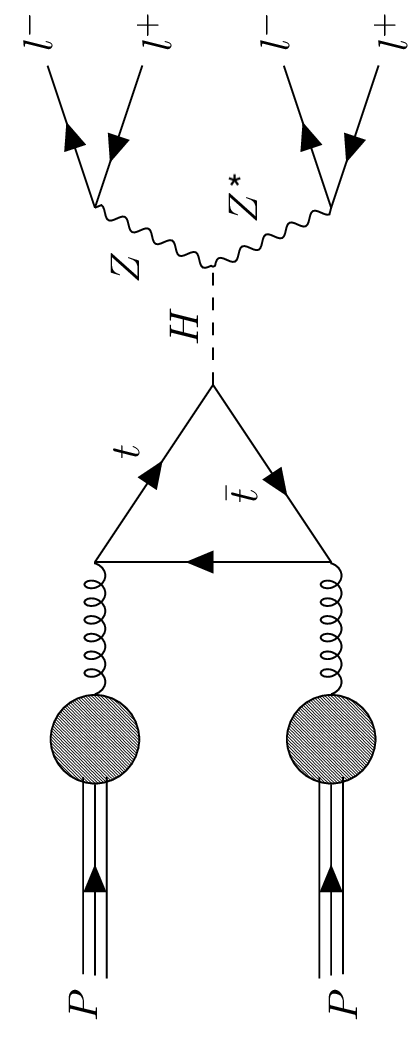
\includegraphics[width=0.43\textwidth, angle = -90]{Figures/FDiagrams/h.png}
            \caption{}
            \label{fig:h}
        \end{subfigure}
    }
    \caption{A collection of examples of Feynman diagrams for the \ac{SM} background processes.
    The diagrams display an example of the processes $Z-jets$ (\ref{fig:z_pjets}), $Diboson(lll)$
    (\ref{fig:wz}), $t\bar{t}$ (\ref{fig:ttbar}), $Diboson(llll)$ (\ref{fig:zz}), $TopOthers$ (\ref{fig:topOthers}),
    $SingleTop$ (\ref{fig:singleTop}), $Diboson(ll)$ (\ref{fig:ww}), $Triboson$ \ref{fig:zzz},
    $W-jets$ (\ref{fig:w_pjets}) and $Higgs$ (\ref{fig:h}).}
    \label{fig:Feynman}
\end{figure}
\newpage
